\paragraph{Метод векторных произведений}
%Каноническое уравнение прямой, заданной по двум точкам $A,B$
%\begin{equation*}
%	\frac{x-x_A}{x_B-x_A} = \frac{y-y_A}{y_B-y_A}
%\end{equation*}
Направляющий вектор прямой заданной по двум точкам $A,B$
\begin{equation*}
	\vec{n} = \begin{pmatrix}
		x_B-x_A\\
		y_B-y_A
	\end{pmatrix}
\end{equation*}
Каждое ребро плоского КЭ можно описать, как часть прямой заданной по двум вершинам этого ребра. Рассмотрим точку $O$, положение которой относительно прямой можно определить с помощью векторного произведения. В зависимости от положения точки векторное произведение будет иметь положительное или отрицательное направление по оси $z$, см. Рисунок \ref{vec_example} (a) и (b) соответственно.
\begin{figure}[H]
	\hfill
	\begin{subfigure}{.45\textwidth}
		\centering
		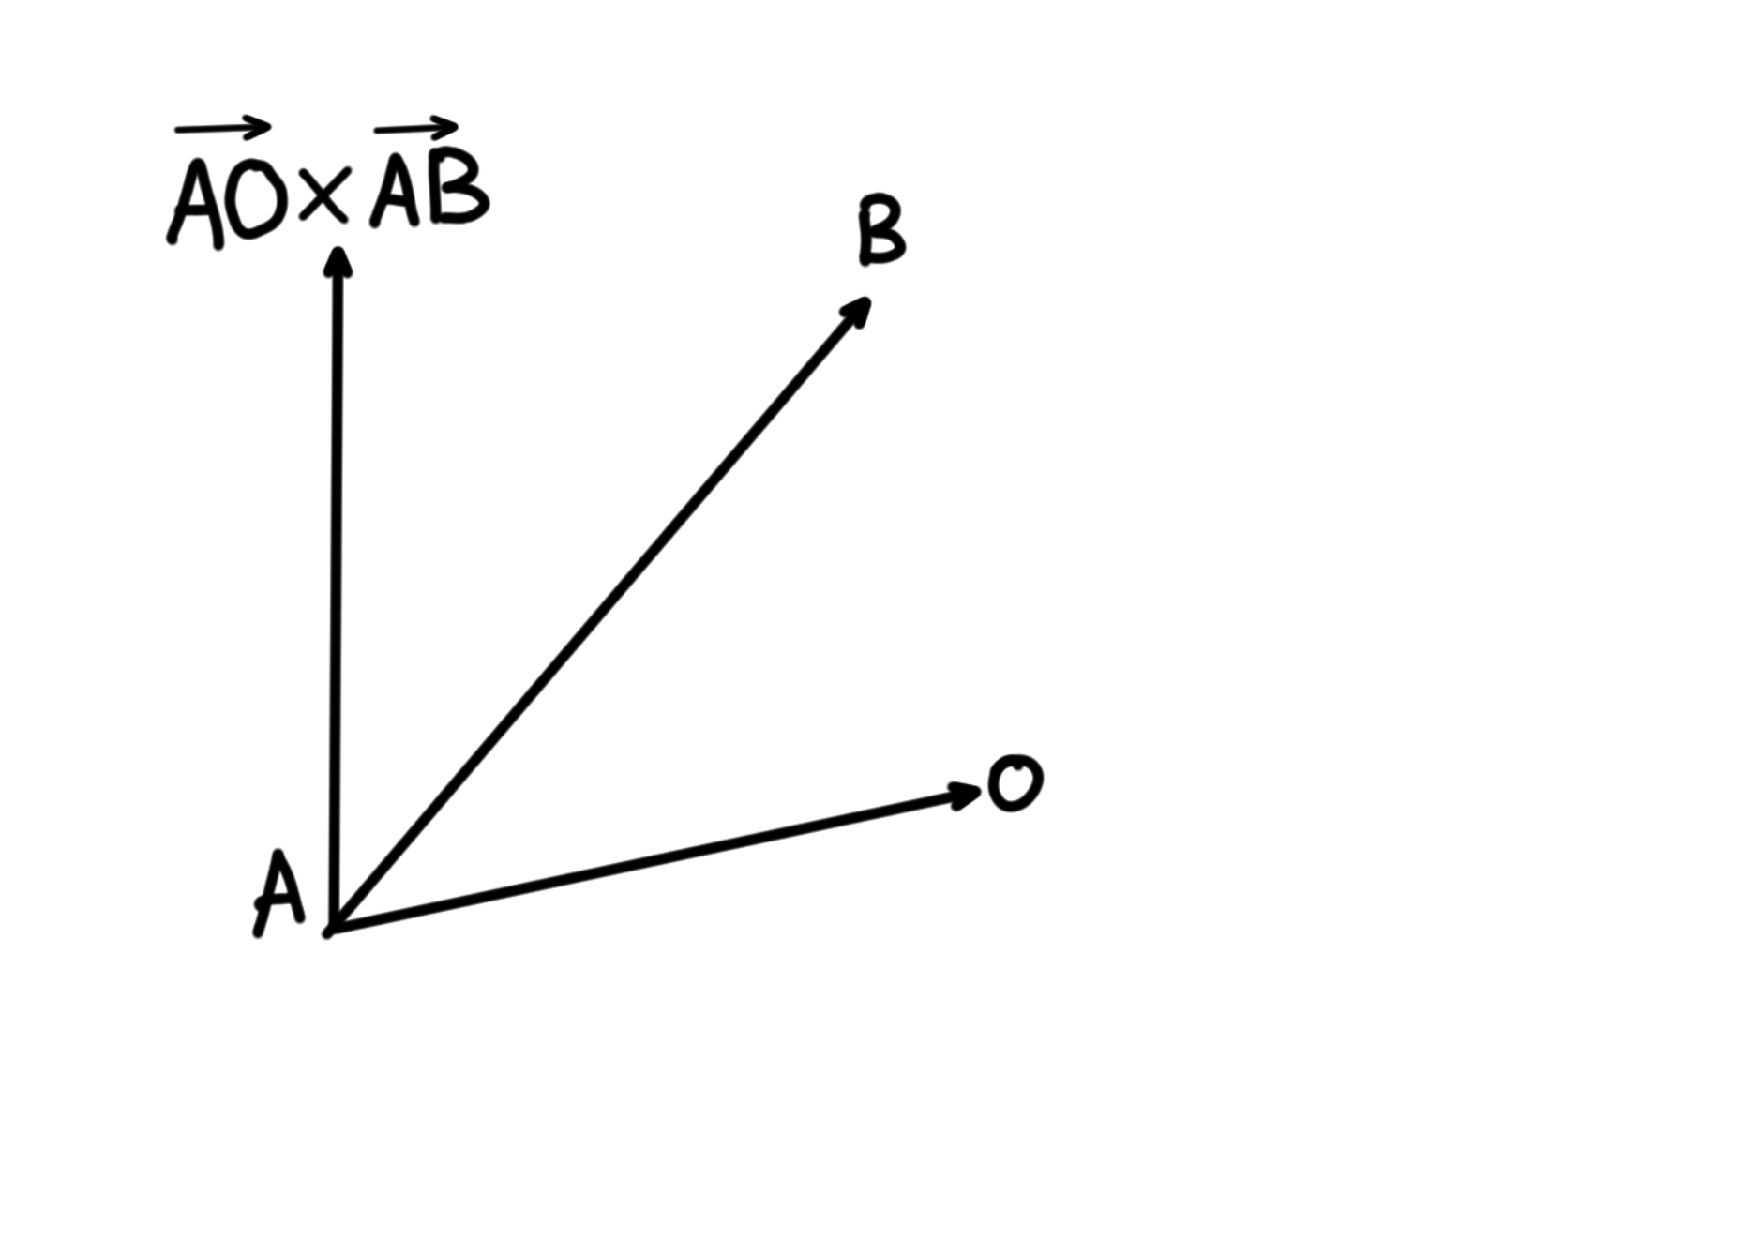
\includegraphics[width=\linewidth,page=1,trim={2cm 5cm 11cm 2cm}]{img/gm}
		\caption{Точка справа от прямой, векторное произведение положительное}
	\end{subfigure}
	\hfill
	\begin{subfigure}{.45\textwidth}
		\centering
		\includegraphics[width=\linewidth,page=2,trim={2cm 0cm 8cm 1cm}]{img/gm}
		\caption{Точка слева от прямой, векторное произведение отрицательное}
	\end{subfigure}
	\hfill
	\caption{Применение векторного произведения для определения положения точки относительно прямой}
	\label{vec_example}
\end{figure}

Просчитав векторное произведение направляющего вектора $\vec{n}$ каждого ребра многоугольника с вектором из первой его вершины в точку $O$, положение которой необходимо определить, можно сделать вывод, о положении точки относительно выпуклого многоугольника. Если точка внутри, то все векторные произведение будут направлены в положительном направлении, иначе точка находится вне многоугольника (см. примеры с параллелепипедом (a) и треугольником (b) на Рисунке \ref{vec_method}).
\begin{figure}[H]
	\hfill
	\begin{subfigure}{.55\textwidth}
		\centering
		\includegraphics[width=\linewidth,page=3,trim={0cm 7cm 3cm 0cm}]{img/gm}
		\caption{Точка внутри параллелепипеда, все векторные произведение направлены в положительном направлении}
	\end{subfigure}
	\hfill
	\begin{subfigure}{.35\textwidth}
		\centering
		\includegraphics[width=\linewidth,page=4,trim={4cm 7cm 12cm 0cm}]{img/gm}
		\caption{Точка вне треугольника, одно из векторных произведений направлено в отрицательном направлении}
	\end{subfigure}
	\hfill
	\caption{Применение векторного произведения для решения задачи принадлежности точки многоугольнику}
	\label{vec_method}
\end{figure}

Таким образом можно определить находится ли точка внутри выпуклого многогранника. Этот метод удобен, так как не ограничивает тип сетки, а в качестве КЭ примет любой n-угольник.
Направляющий вектор прямой имеет вид:
\begin{equation*}
	\vec{AB} = \vec n = \begin{pmatrix}
		x_B - x_A\\
		y_B - y_A\\
		0
	\end{pmatrix}.
\end{equation*}
Вектор $AO$ задаётся аналогично:
\begin{equation*}
	\vec {AO} = \begin{pmatrix}
		x_O - x_A\\
		y_O - y_A\\
		0
	\end{pmatrix}
\end{equation*}
Тогда векторное произведение $\vec{AO}\times\vec{AB}$ легко посчитать следующим образом:
\begin{multline*}
	\vec{AO}\times\vec{AB} = \left|\begin{array}{ccc}
		\vec{x} & \vec{y} & \vec{z} \\
		x_B - x_A & y_B - y_A & 0 \\
		x_O - x_A & y_O - y_A & 0 \\
	\end{array}\right| =\\= \vec{z}\cdot\left(\left(x_B - x_A\right)\cdot\left(y_O - y_A\right) - \left(y_B - y_A\right)\cdot\left(x_O - x_A\right)\right)
\end{multline*}
Следовательно выражение $\left(x_B - x_A\right)\cdot\left(y_O - y_A\right) - \left(y_B - y_A\right)\cdot\left(x_O - x_A\right)$ в зависимости от его знака будет определять положение точки. Код программы для определения положения точки относительно прямой:
\lstinputlisting[language=C++, firstline=16, lastline=27]{current-lines/src/Geometry/Line.cpp}

Код программы для определения положения точки относительно конечного элемента:
\lstinputlisting[language=C++, firstline=147, lastline=155]{current-lines/src/Element/Element.cpp}
Здесь программа циклично проверяет положение точки относительно каждого ребра. Также дополнительно добавлена проверка того, что точка находится в диапазоне значений $x$ и $y$ для данного элемента. Эта проверка позволяет сразу сказать, что точка лежит вне КЭ, если она находится очень далеко от него.